\documentclass[11pt,a4paper]{article}

% ── Packages ──────────────────────────────────────────────────────────────────
\usepackage{amsmath,amsthm,amssymb,mathtools}
\usepackage[margin=2.5cm]{geometry}
\usepackage{hyperref}
\usepackage{enumitem}
\usepackage{booktabs}
\usepackage{xcolor}
\usepackage{tikz}
\usetikzlibrary{arrows.meta,positioning,calc,decorations.pathmorphing}
\usepackage{algorithm}
\usepackage{algpseudocode}
\usepackage{thmtools}

% ── Theorem environments ─────────────────────────────────────────────────────
\newtheorem{theorem}{Theorem}[section]
\newtheorem{proposition}[theorem]{Proposition}
\newtheorem{lemma}[theorem]{Lemma}
\newtheorem{corollary}[theorem]{Corollary}
\theoremstyle{definition}
\newtheorem{definition}[theorem]{Definition}
\newtheorem{example}[theorem]{Example}
\newtheorem{remark}[theorem]{Remark}

% ── Custom commands ──────────────────────────────────────────────────────────
\newcommand{\KL}{\mathrm{D}_{\mathrm{KL}}}
\newcommand{\E}{\mathbb{E}}
\newcommand{\R}{\mathbb{R}}
\newcommand{\bmu}{\boldsymbol{\mu}}
\newcommand{\bsigma}{\boldsymbol{\sigma}}
\newcommand{\btheta}{\boldsymbol{\theta}}
\newcommand{\cF}{\mathcal{F}}
\newcommand{\cG}{\mathcal{G}}
\newcommand{\cL}{\mathcal{L}}
\DeclareMathOperator*{\argmin}{arg\,min}
\DeclareMathOperator*{\argmax}{arg\,max}

\hypersetup{
  colorlinks=true,
  linkcolor=blue!70!black,
  citecolor=green!50!black,
  urlcolor=blue!60!black
}

% ══════════════════════════════════════════════════════════════════════════════
\begin{document}

\begin{center}
  {\LARGE \textbf{Active Inference and the Free Energy Principle:}}\\[4pt]
  {\LARGE \textbf{Mathematical Foundations for Agentic AI}}\\[12pt]
  {\large Research Notes --- ETH Zurich ML Lecture Series}\\[8pt]
  {\normalsize Computational Neuroscience \& Machine Learning}\\[4pt]
  {\small Spring 2026}
\end{center}

\vspace{1em}

\begin{abstract}
These notes provide a mathematically rigorous introduction to the Free Energy
Principle (FEP) and Active Inference, a unified framework originating in
computational neuroscience that casts perception, learning, and action as
variational inference.  We derive variational free energy from first
principles, formalize Markov blankets and their controversies, develop the
Expected Free Energy objective for planning, and connect these ideas to modern
agentic AI---including reinforcement learning, large language models, and
multi-agent systems.  We present the framework's critics fairly, survey open
problems, and provide an annotated bibliography for further study.
\end{abstract}

\tableofcontents
\newpage

% ══════════════════════════════════════════════════════════════════════════════
\section{Introduction and Historical Context}
\label{sec:intro}

The \textbf{Free Energy Principle} (FEP), developed primarily by Karl Friston
at University College London beginning in the mid-2000s, proposes that any
self-organizing system that persists in a changing environment must minimize a
quantity called \emph{variational free energy}---or equivalently, maximize
Bayesian model evidence.  From this single imperative, one can derive
perception (updating beliefs about the world), action (changing the world to
match predictions), learning (adjusting generative model parameters), and
attention (adjusting the precision of predictions).

\textbf{Active Inference} (AIF) is the process theory that operationalizes the
FEP.  Where the FEP is a principle about what self-organizing systems
\emph{must} do, active inference specifies \emph{how} they do it: by selecting
policies (action sequences) that minimize \emph{expected free energy}, a
functional that naturally balances exploration and exploitation.

\paragraph{Why should ML researchers care?}
\begin{enumerate}[leftmargin=2em]
  \item Active inference provides a principled alternative to reward-based RL,
    deriving curiosity-driven exploration from first principles rather than
    bolting it on as an auxiliary loss.
  \item The mathematics connects directly to variational autoencoders (VAEs),
    Bayesian neural networks, and planning-as-inference.
  \item The framework offers a natural language for multi-agent coordination,
    hierarchical planning, and embodied AI.
  \item Recent work on Bayesian mechanics (Ramstead, Da Costa et al.) is
    building a rigorous mathematical physics of belief-updating systems.
\end{enumerate}

\paragraph{Outline.}  Section~\ref{sec:vfe} derives variational free energy.
Section~\ref{sec:mb} covers Markov blankets and their controversies.
Section~\ref{sec:aif} develops active inference and expected free energy.
Section~\ref{sec:sophisticated} introduces sophisticated inference.
Section~\ref{sec:bayesmech} covers Bayesian mechanics.
Section~\ref{sec:genmodels} surveys generative models.
Section~\ref{sec:connections} draws connections to modern agentic AI.
Section~\ref{sec:controversies} presents critiques.
Section~\ref{sec:open} lists open problems.
Section~\ref{sec:bib} provides an annotated bibliography.


% ══════════════════════════════════════════════════════════════════════════════
\section{Variational Free Energy}
\label{sec:vfe}

\subsection{Derivation from Bayes' Theorem}

We begin with a generative model $p(o, \theta)$ that specifies a joint
distribution over observations $o$ and latent variables (hidden states,
parameters, etc.)\ $\theta$.  Exact Bayesian inference requires computing:
\begin{equation}
  p(\theta \mid o) = \frac{p(o \mid \theta)\, p(\theta)}{p(o)},
  \qquad
  p(o) = \int p(o \mid \theta)\, p(\theta)\, d\theta.
  \label{eq:bayes}
\end{equation}
The marginal likelihood (model evidence) $p(o)$ is typically intractable.

\paragraph{Step 1: Introduce a recognition density.}
Let $q(\theta)$ be an approximate posterior (recognition density) over $\theta$.
Consider the log model evidence:
\begin{equation}
  \ln p(o) = \ln \int p(o, \theta)\, d\theta.
  \label{eq:logev}
\end{equation}

\paragraph{Step 2: Apply Jensen's inequality (or direct decomposition).}
We can decompose $\ln p(o)$ exactly.  For any $q(\theta)$:
\begin{align}
  \ln p(o)
  &= \int q(\theta) \ln p(o)\, d\theta
  \notag \\
  &= \int q(\theta) \ln \frac{p(o, \theta)}{p(\theta \mid o)}\, d\theta
  \notag \\
  &= \int q(\theta) \ln \frac{p(o, \theta)}{q(\theta)}
     \cdot \frac{q(\theta)}{p(\theta \mid o)}\, d\theta
  \notag \\
  &= \underbrace{\int q(\theta) \ln \frac{p(o, \theta)}{q(\theta)}\, d\theta}_{
       -\cF[q, o] \;\text{(negative free energy = ELBO)}}
   + \underbrace{\int q(\theta) \ln \frac{q(\theta)}{p(\theta \mid o)}\, d\theta}_{
       \KL[q(\theta) \| p(\theta \mid o)] \;\geq\; 0}.
  \label{eq:decomp}
\end{align}

\begin{definition}[Variational Free Energy]
The \textbf{variational free energy} is defined as:
\begin{equation}
  \boxed{
  \cF[q, o] \;=\; -\int q(\theta) \ln \frac{p(o, \theta)}{q(\theta)}\, d\theta
  \;=\; \KL\bigl[q(\theta) \,\|\, p(\theta)\bigr]
       - \E_{q}\bigl[\ln p(o \mid \theta)\bigr].
  }
  \label{eq:vfe}
\end{equation}
\end{definition}

\paragraph{Step 3: The two decompositions.}
Equation~\eqref{eq:vfe} admits two useful decompositions:

\medskip
\noindent
\textbf{(a) Complexity -- Accuracy:}
\begin{equation}
  \cF = \underbrace{\KL[q(\theta) \| p(\theta)]}_{\text{Complexity}}
      - \underbrace{\E_q[\ln p(o \mid \theta)]}_{\text{Accuracy}}.
  \label{eq:ca}
\end{equation}
Minimizing $\cF$ balances fitting the data (accuracy) against deviating from
the prior (complexity).  This is Occam's razor in variational form.

\medskip
\noindent
\textbf{(b) Energy -- Entropy:}
\begin{equation}
  \cF = \underbrace{\E_q[-\ln p(o, \theta)]}_{\text{Energy}}
      - \underbrace{H[q(\theta)]}_{\text{Entropy}},
  \label{eq:ee}
\end{equation}
where $H[q] = -\E_q[\ln q(\theta)]$.  This form connects to statistical
physics: $\cF$ is literally a free energy in the thermodynamic sense when $q$
is interpreted as a Boltzmann distribution.

\paragraph{Step 4: Connection to model evidence.}
From~\eqref{eq:decomp}:
\begin{equation}
  \cF = -\ln p(o) + \KL[q(\theta) \| p(\theta \mid o)].
  \label{eq:bound}
\end{equation}
Since $\KL \geq 0$, we have $\cF \geq -\ln p(o)$, i.e., $-\cF \leq \ln p(o)$
(the ELBO).  Minimizing $\cF$ over $q$ simultaneously: (i) tightens the bound,
and (ii) drives $q(\theta) \to p(\theta \mid o)$.

\subsection{Connection to Variational Autoencoders}

The VAE objective is precisely the negative free energy (the ELBO):
\begin{equation}
  \cL_{\text{VAE}}(\phi, \psi; o)
  = \E_{q_\phi(z \mid o)}[\ln p_\psi(o \mid z)]
  - \KL[q_\phi(z \mid o) \| p(z)]
  = -\cF.
\end{equation}
The encoder $q_\phi$ is the recognition model; the decoder $p_\psi$ is the
generative model.  Active inference extends this by closing the loop: the
``decoder'' generates predictions about sensory data, and the agent \emph{acts}
to make those predictions come true.

\subsection{Free Energy Minimization as a Universal Objective}

\begin{proposition}
Under the FEP, the following are all instances of free energy minimization:
\begin{enumerate}[leftmargin=2em]
  \item \textbf{Perception:} $q^* = \argmin_q \cF[q, o]$ (update beliefs given
    observations).
  \item \textbf{Action:} $a^* = \argmin_a \cF[q, o(a)]$ (change observations
    to reduce surprise).
  \item \textbf{Learning:} $\psi^* = \argmin_\psi \cF[q, o; \psi]$ (adjust
    generative model parameters).
  \item \textbf{Attention:} Optimize the precision (inverse variance) of
    prediction errors.
\end{enumerate}
\end{proposition}


% ══════════════════════════════════════════════════════════════════════════════
\section{Markov Blankets}
\label{sec:mb}

\subsection{Definition and Partition}

\begin{definition}[Markov Blanket]
Given a set of random variables $x = (\mu, s, a, \eta)$, the \textbf{Markov
blanket} of the internal states $\mu$ is the set $b = (s, a)$ such that $\mu$
and $\eta$ are conditionally independent given $b$:
\begin{equation}
  \mu \perp\!\!\!\perp \eta \;\mid\; b = (s, a).
\end{equation}
Here:
\begin{itemize}[leftmargin=2em]
  \item $\mu$ = internal states (the system's ``beliefs''),
  \item $s$ = sensory states (blanket states influenced by external states),
  \item $a$ = active states (blanket states influenced by internal states),
  \item $\eta$ = external (environmental) states.
\end{itemize}
\end{definition}

The Markov blanket induces a statistical boundary: internal states can only
``know about'' external states through sensory states, and can only
``influence'' external states through active states.

\begin{figure}[h]
\centering
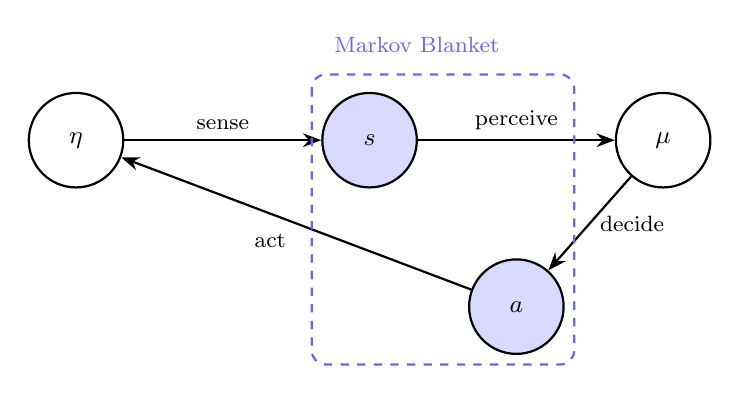
\begin{tikzpicture}[
  node distance=2.5cm,
  state/.style={circle, draw, thick, minimum size=1.2cm, font=\small},
  blanket/.style={state, fill=blue!15},
  >=Stealth
]
  \node[state] (eta) {$\eta$};
  \node[blanket, right=of eta] (s) {$s$};
  \node[state, right=of s] (mu) {$\mu$};
  \node[blanket, below=1.5cm of $(s)!0.5!(mu)$] (a) {$a$};

  \draw[->, thick] (eta) -- (s) node[midway, above, font=\footnotesize] {sense};
  \draw[->, thick] (s) -- (mu) node[midway, above, font=\footnotesize] {perceive};
  \draw[->, thick] (mu) -- (a) node[midway, right, font=\footnotesize] {decide};
  \draw[->, thick] (a) -- (eta) node[midway, below left, font=\footnotesize] {act};

  % Blanket box
  \draw[dashed, blue!60, thick, rounded corners=5pt]
    ($(s.north west)+(-0.3,0.4)$) rectangle ($(a.south east)+(0.3,-0.3)$);
  \node[blue!60, font=\footnotesize] at ($(s.north)+(0.6,0.6)$) {Markov Blanket};
\end{tikzpicture}
\caption{The four-way partition $x = (\mu, s, a, \eta)$ with the Markov blanket
$b = (s, a)$ separating internal from external states.}
\label{fig:mb}
\end{figure}

\subsection{Langevin Dynamics and the FEP}

Friston's formulation starts with a Langevin (stochastic differential) equation
on the full state space:
\begin{equation}
  \dot{x} = f(x) + \omega, \qquad \omega \sim \mathcal{N}(0, 2\Gamma),
  \label{eq:langevin}
\end{equation}
where $f(x)$ is the flow and $\Gamma$ is the diffusion tensor.  At the
nonequilibrium steady state (NESS), the dynamics admit a decomposition:
\begin{equation}
  f(x) = (\Gamma - Q)\, \nabla \ln p(x),
\end{equation}
where $Q = -Q^\top$ is a solenoidal (antisymmetric) matrix encoding
circulation, and $\Gamma$ is the symmetric part encoding dissipation.  This is
the \textbf{Helmholtz decomposition} of the flow.

Given the Markov blanket partition, one can show that internal states
$\mu$ parameterize a density $q_\mu(\eta) \approx p(\eta \mid b)$, so that the
internal dynamics effectively perform (approximate) Bayesian inference on
external states.  This is the core claim of the FEP: the internal states of any
Markov-blanketed system \emph{look as if} they are performing inference.

\subsection{The Controversy: Critiques of Markov Blankets under the FEP}
\label{sec:mb_controversy}

The application of Markov blankets in the FEP has generated significant
debate.  We present both sides.

\paragraph{The Critiques.}

\begin{enumerate}[leftmargin=2em]
  \item \textbf{Biehl et al.\ (2021):} ``A Technical Critique of Some Parts of
    the Free Energy Principle.''  The authors argue that:
    \begin{itemize}
      \item The claim that internal states parameterize a density over external
        states relies on an unjustified identification between the \emph{mode}
        of the conditional distribution $p(\eta \mid b)$ and a ``belief.''
      \item The Markov blanket formalism in continuous-time dynamics does not
        straightforwardly yield the conditional independence structure assumed
        in graphical model theory.
      \item The ``as if'' inference claim is not falsifiable: any system with a
        stationary distribution can be redescribed in these terms.
    \end{itemize}

  \item \textbf{Bruineberg et al.\ (2022):} ``The Emperor's New Markov
    Blankets'' argues that:
    \begin{itemize}
      \item There is a conflation between \emph{Pearl blankets} (conditional
        independence in a Bayesian network) and \emph{Friston blankets}
        (partitions of a Langevin system at NESS).
      \item Pearl blankets are properties of a graph; Friston blankets are
        properties of a dynamical system.  The two do not trivially map onto
        each other.
      \item The claim that ``everything has a Markov blanket'' is either trivially
        true (any partition defines conditional independence structure) or
        substantively false (not every system has the right kind of partition).
    \end{itemize}
\end{enumerate}

\paragraph{The Defense.}

\begin{enumerate}[leftmargin=2em]
  \item \textbf{Friston, Da Costa, and Parr} have responded that the critics
    conflate different levels of description.  The FEP does not claim that
    every system literally performs Bayesian inference, but rather that its
    dynamics can be \emph{described as if} it does---a modeling stance, not an
    ontological claim.
  \item \textbf{Da Costa et al.\ (2021)} formalized Bayesian mechanics on
    nonequilibrium steady-state systems, providing conditions under which the
    ``as if'' interpretation holds rigorously.  They distinguish between a
    \emph{particular partition} (the Markov blanket exists as a dynamical
    structure) and the interpretation layer.
  \item \textbf{Ramstead et al.\ (2023)} introduced the concept of a
    \emph{sparse coupling} condition that replaces the graphical-model Markov
    blanket with a dynamical-systems notion, partially addressing Bruineberg
    et al.'s concerns.
\end{enumerate}

\begin{remark}
For the working ML researcher, the practical takeaway is: the Markov blanket
formalism is a powerful \emph{modeling assumption} for designing agents.
Whether it constitutes a ``law of nature'' is a philosophical question that
does not affect the utility of active inference as an algorithm.
\end{remark}


% ══════════════════════════════════════════════════════════════════════════════
\section{Active Inference}
\label{sec:aif}

\subsection{Perception and Action as Inference}

In active inference, an agent has a generative model
$p(o_{1:T}, s_{1:T}, \pi)$ over observations $o$, hidden states $s$, and
policies $\pi$ (sequences of actions).  At each time step, the agent:

\begin{enumerate}[leftmargin=2em]
  \item \textbf{Perceives:} Updates beliefs over hidden states by minimizing
    variational free energy given new observations:
    \begin{equation}
      q(s_t) = \argmin_{q} \cF[q, o_t].
    \end{equation}
  \item \textbf{Plans:} Evaluates policies by computing expected free energy
    (see below) and selects actions accordingly.
  \item \textbf{Acts:} Executes the action prescribed by the selected policy,
    generating new observations.
  \item \textbf{Learns:} Updates model parameters to reduce long-run free
    energy.
\end{enumerate}

\subsection{Expected Free Energy}
\label{sec:efe}

The key innovation of active inference for planning is the \textbf{Expected
Free Energy} (EFE), denoted $\cG(\pi)$.

\begin{definition}[Expected Free Energy]
For a policy $\pi$, the expected free energy at future time $\tau$ is:
\begin{equation}
  \cG(\pi, \tau) = \E_{\tilde{q}}\bigl[
    \ln q(s_\tau \mid \pi) - \ln p(o_\tau, s_\tau \mid \pi)
  \bigr],
  \label{eq:efe}
\end{equation}
where $\tilde{q} = q(o_\tau, s_\tau \mid \pi)$ is the predictive distribution
under the approximate posterior.
\end{definition}

\paragraph{Decomposition into epistemic and pragmatic value.}
\begin{align}
  \cG(\pi, \tau)
  &= \underbrace{-\E_{\tilde{q}}\bigl[
       \KL[q(s_\tau \mid o_\tau, \pi) \| q(s_\tau \mid \pi)]
     \bigr]}_{\text{Epistemic value (neg.\ information gain)}}
  + \underbrace{\E_{\tilde{q}}\bigl[
       \ln q(o_\tau \mid \pi) - \ln p(o_\tau)
     \bigr]}_{\text{Pragmatic value (neg.\ expected log preference)}}.
  \notag
\end{align}

Rewriting with clearer signs:
\begin{equation}
  \boxed{
  \cG(\pi) = -\underbrace{\text{Information Gain}}_{\text{Exploration}}
           \;-\; \underbrace{\text{Pragmatic Value}}_{\text{Exploitation}}.
  }
  \label{eq:efe_decomp}
\end{equation}

\begin{itemize}[leftmargin=2em]
  \item \textbf{Information Gain} (epistemic value): the expected reduction in
    uncertainty about hidden states after observing the outcome of a policy.
    This drives \emph{exploration}---the agent seeks out informative observations.
  \item \textbf{Pragmatic Value}: how well the predicted observations align
    with the agent's preferred observations $p(o_\tau)$ (prior preferences).
    This drives \emph{exploitation}---the agent pursues goals.
\end{itemize}

\paragraph{Policy selection.}
Policies are selected via a softmax over negative EFE:
\begin{equation}
  p(\pi) = \sigma(-\gamma \cG(\pi))
  = \frac{\exp(-\gamma \cG(\pi))}{\sum_{\pi'} \exp(-\gamma \cG(\pi'))},
  \label{eq:policy_select}
\end{equation}
where $\gamma > 0$ is a precision (inverse temperature) parameter.

\subsection{Contrast with Reinforcement Learning}

\begin{table}[h]
\centering
\small
\begin{tabular}{@{}lll@{}}
\toprule
\textbf{Aspect} & \textbf{Active Inference} & \textbf{Reinforcement Learning} \\
\midrule
Objective & Minimize expected free energy & Maximize expected cumulative reward \\
Exploration & Intrinsic (information gain) & Extrinsic (epsilon-greedy, UCB, etc.) \\
Reward & Prior preferences over observations & Externally defined reward function \\
Model & Generative model (required) & Optional (model-free or model-based) \\
Optimality & Bayes-optimal given model & Bellman-optimal given MDP \\
Curiosity & First-class citizen & Auxiliary bonus (e.g., ICM, RND) \\
Multi-objective & Natural (prior preferences) & Requires reward shaping \\
\bottomrule
\end{tabular}
\caption{Active inference vs.\ reinforcement learning.}
\label{tab:aif_rl}
\end{table}

\begin{remark}
Active inference and RL are not incompatible.  When information gain is zero
(no epistemic uncertainty) and we identify $\ln p(o) = r(o)$, the EFE reduces
to expected reward, and active inference recovers KL-regularized RL (similar to
SAC/MaxEnt RL).  The key difference is that exploration is derived, not added.
\end{remark}

\subsection{The Full Active Inference Loop}

\begin{algorithm}[h]
\caption{Discrete Active Inference Agent (one time step)}
\label{alg:aif}
\begin{algorithmic}[1]
\Require Generative model $p(o_{1:T}, s_{1:T}, \pi)$, current beliefs $q(s_t)$
\State Observe $o_t$
\State \textbf{Perception:} Update $q(s_t) \leftarrow \argmin_q \cF[q, o_t]$
  \Comment{State estimation}
\For{each policy $\pi \in \Pi$}
  \State Compute $\cG(\pi) = \sum_{\tau > t} \cG(\pi, \tau)$
  \Comment{Expected free energy}
\EndFor
\State \textbf{Policy selection:} Sample $\pi^* \sim \sigma(-\gamma\, \cG(\pi))$
\State \textbf{Action:} Execute $a_t = \pi^*(t)$
  \Comment{First action of selected policy}
\State \textbf{Learning:} Update model parameters to reduce $\cF$
  \Comment{Optional}
\end{algorithmic}
\end{algorithm}


% ══════════════════════════════════════════════════════════════════════════════
\section{Sophisticated Inference}
\label{sec:sophisticated}

Standard active inference evaluates policies by summing EFE over future time
steps, treating each step independently.  \textbf{Sophisticated inference}
(Friston et al., 2021) extends this by introducing \emph{recursive policy
evaluation}: the agent considers what it would \emph{believe and do} in the
future, given possible observations.

\subsection{Recursive Evaluation}

At each decision point, the sophisticated agent:
\begin{enumerate}[leftmargin=2em]
  \item Generates possible future observations $o_{\tau+1}$ under each policy.
  \item For each possible observation, computes the updated beliefs
    $q(s_{\tau+1} \mid o_{\tau+1})$.
  \item Given those updated beliefs, recursively evaluates what policy would
    be selected at time $\tau+1$, and so on.
  \item The expected free energy is computed over the full tree of future
    contingencies.
\end{enumerate}

Formally, the sophisticated EFE at depth $d$ is:
\begin{equation}
  \cG^{(d)}(\pi, \tau) = \cG(\pi, \tau)
  + \E_{\tilde{q}(o_{\tau+1} \mid \pi)}\bigl[
    \min_{\pi'} \cG^{(d-1)}(\pi', \tau+1 \mid o_{\tau+1})
  \bigr],
  \label{eq:sophisticated}
\end{equation}
with $\cG^{(0)} = \cG$ (the standard EFE).

\subsection{Connection to MCTS and AlphaZero}

Sophisticated inference bears a structural resemblance to Monte Carlo Tree
Search (MCTS):
\begin{itemize}[leftmargin=2em]
  \item Both build a tree of future contingencies.
  \item Both evaluate leaf nodes with a value function (EFE plays this role).
  \item Both propagate values back up the tree.
\end{itemize}

The key differences:
\begin{itemize}[leftmargin=2em]
  \item MCTS uses rollouts or a learned value network; sophisticated inference
    uses the generative model's predictive distributions.
  \item AlphaZero's value/policy networks can be seen as amortized versions
    of the recursive EFE computation.
  \item Sophisticated inference naturally handles partial observability
    (POMDPs), while standard MCTS typically assumes full state observability.
\end{itemize}

\begin{remark}
Champion et al.\ (2022) have shown that deep active inference agents using
tree search can achieve competitive performance with AlphaZero-style agents in
certain domains, while requiring less training data due to the built-in
epistemic drive.
\end{remark}


% ══════════════════════════════════════════════════════════════════════════════
\section{Bayesian Mechanics}
\label{sec:bayesmech}

\textbf{Bayesian mechanics} is a recent program (Ramstead, Da Costa, Sakthivadivel,
Friston et al., 2023--2025) that aims to place the FEP on rigorous
mathematical-physics foundations.

\subsection{The Core Idea}

Bayesian mechanics studies the mechanics of systems that can be described as
performing inference---specifically, systems whose internal states parameterize
probability distributions over external states.  The central question: given a
particular partition (a Markov blanket structure) of a dynamical system, what
are the equations of motion for the ``beliefs'' encoded by internal states?

\subsection{Path Integral Formulation}

Following the Feynman--Kac approach, one can express the marginal likelihood
over a trajectory of observations $o_{0:T}$ as a path integral:
\begin{equation}
  p(o_{0:T}) = \int \mathcal{D}[s_{0:T}]\;
  p(o_{0:T} \mid s_{0:T})\, p(s_{0:T}),
  \label{eq:path_integral}
\end{equation}
where $\mathcal{D}[s_{0:T}]$ denotes integration over all possible hidden state
trajectories.  The variational free energy then becomes a functional over
trajectory space:
\begin{equation}
  \cF[q] = \KL\bigl[q(s_{0:T}) \,\|\, p(s_{0:T})\bigr]
          - \E_q\bigl[\ln p(o_{0:T} \mid s_{0:T})\bigr].
\end{equation}

\subsection{Connection to Jaynes' Maximum Entropy}

Jaynes' MaxEnt principle states that the least biased distribution consistent
with known constraints is the one with maximum entropy.  Bayesian mechanics
connects this to the FEP:

\begin{proposition}
At the NESS of a Langevin system, the steady-state density $p_\infty(x)$
maximizes entropy subject to the constraint that the expected energy is fixed.
The internal states' dynamics then minimize a free energy functional that is
formally identical to Jaynes' MaxEnt objective.
\end{proposition}

This provides a deep link between information geometry, statistical physics,
and the FEP.

\subsection{Hamilton's Equations for Belief Systems}

Da Costa and colleagues have shown that, under certain regularity conditions,
the dynamics of belief-parameterizing internal states can be written in
Hamiltonian form:
\begin{equation}
  \dot{\mu}_i = \frac{\partial \mathcal{H}}{\partial \nu_i},
  \qquad
  \dot{\nu}_i = -\frac{\partial \mathcal{H}}{\partial \mu_i} + \text{dissipation},
  \label{eq:hamilton_belief}
\end{equation}
where $\mu_i$ are the ``belief coordinates,'' $\nu_i$ are conjugate momenta,
and $\mathcal{H}$ is a Hamiltonian that plays the role of free energy.  The
dissipation term reflects the irreversible, entropy-producing character of
inference in open systems.

\begin{remark}
This is a genuinely new result: it says that belief dynamics obey a
generalization of Hamilton's equations from classical mechanics, providing a
``physics of inference.''  The solenoidal (conservative) part drives
oscillations and cycles in belief space; the dissipative part drives convergence
to the posterior.
\end{remark}


% ══════════════════════════════════════════════════════════════════════════════
\section{Generative Models for Active Inference}
\label{sec:genmodels}

Active inference is model-based by construction.  The choice of generative
model determines the agent's representational capacity and computational
requirements.

\subsection{Discrete State-Space Models}

\paragraph{Hidden Markov Models (HMMs).}
The simplest generative model:
\begin{align}
  p(s_t \mid s_{t-1}) &= \mathbf{B}\, \delta_{s_{t-1}},
  &\text{(transition model)} \\
  p(o_t \mid s_t) &= \mathbf{A}\, \delta_{s_t},
  &\text{(observation model)}
\end{align}
where $\mathbf{A}$ and $\mathbf{B}$ are categorical probability matrices.
Perception reduces to Bayesian filtering; planning to evaluating a finite set
of policies.

\paragraph{POMDPs.}
Active inference POMDPs extend HMMs with policy-dependent transitions:
\begin{equation}
  p(o_{1:T}, s_{1:T} \mid \pi) = p(s_1) \prod_{t=1}^{T} p(o_t \mid s_t)
  \prod_{t=2}^{T} p(s_t \mid s_{t-1}, \pi(t-1)).
\end{equation}
The agent maintains beliefs $q(s_t \mid \pi)$ and selects policies by
minimizing EFE.  This is the formulation implemented in the \texttt{pymdp}
library (Heins et al., 2022).

\subsection{Continuous State-Space Models}

For continuous domains, the generative model takes the form of stochastic
differential equations:
\begin{align}
  ds &= f(s, a)\, dt + \sigma_s\, dW_s, \\
  o &= g(s) + \sigma_o\, \epsilon,
\end{align}
where $f$ is the state dynamics, $g$ is the observation function, and $W_s$,
$\epsilon$ are Wiener processes / noise.  Inference proceeds via
\textbf{generalized filtering} or \textbf{predictive coding}, which can be
seen as gradient descent on free energy in generalized coordinates of motion
(position, velocity, acceleration, \ldots).

\subsection{Deep Active Inference}

Recent work replaces the matrices $\mathbf{A}$, $\mathbf{B}$ with neural
networks:
\begin{itemize}[leftmargin=2em]
  \item \textbf{Deep generative models:} The observation model $p_\psi(o \mid s)$
    is a neural network decoder; the recognition model $q_\phi(s \mid o)$ is a
    neural network encoder.  This yields a VAE-like architecture embedded in an
    active inference loop.
  \item \textbf{Transition models:} $p_\xi(s_{t+1} \mid s_t, a_t)$ can be a
    recurrent or transformer-based model (``world model'').
  \item \textbf{Policy networks:} $q_\omega(\pi)$ amortizes policy selection,
    analogous to the actor in actor-critic methods.
\end{itemize}

\subsection{Hybrid and Hierarchical Models}

\textbf{Pezzulo and colleagues} have developed hierarchical active inference
models where:
\begin{itemize}[leftmargin=2em]
  \item Higher levels operate on slower timescales and more abstract state spaces.
  \item Lower levels operate on faster timescales and concrete sensorimotor
    representations.
  \item Each level minimizes its own free energy, with top-down predictions and
    bottom-up prediction errors propagating between levels.
\end{itemize}
This mirrors the hierarchical structure of the cortex and provides a principled
approach to temporal abstraction (cf.\ options in hierarchical RL).


% ══════════════════════════════════════════════════════════════════════════════
\section{Connections to Modern Agentic AI}
\label{sec:connections}

\subsection{Active Inference vs.\ Deep RL}

Beyond the conceptual differences in Table~\ref{tab:aif_rl}, recent empirical
work has compared active inference agents with RL baselines:

\begin{itemize}[leftmargin=2em]
  \item In structured, partially observable environments, active inference
    agents tend to learn faster due to epistemic drive (built-in curiosity).
  \item In high-dimensional environments with large action spaces, deep RL
    agents currently outperform active inference agents due to better scaling
    of function approximation.
  \item Hybrid approaches (e.g., using EFE as an intrinsic reward in an RL
    framework) show promise.
\end{itemize}

\subsection{Large Language Models Through the Free Energy Lens}

LLMs can be interpreted through the FEP framework:
\begin{itemize}[leftmargin=2em]
  \item \textbf{Next-token prediction is free energy minimization:} The
    training objective $-\sum_t \ln p_\theta(x_t \mid x_{<t})$ is the negative
    log-likelihood, which is the accuracy term of free energy (with implicit
    complexity regularization via weight decay, dropout, etc.).
  \item \textbf{In-context learning as inference:} The context window acts as
    a form of approximate Bayesian inference---the model implicitly conditions
    on context to update its ``beliefs'' about the task.
  \item \textbf{Agentic LLMs:} When LLMs are equipped with tools, memory, and
    planning capabilities, they begin to resemble active inference agents with
    deep generative models.  The key missing ingredient is typically the
    epistemic drive---current agentic LLMs do not systematically seek
    information to reduce uncertainty.
\end{itemize}

\subsection{Robotics and Embodied AI}

Active inference has been applied to:
\begin{itemize}[leftmargin=2em]
  \item Robot navigation and SLAM (simultaneous localization and mapping),
    where the epistemic drive naturally leads to frontier exploration.
  \item Manipulation tasks, where predictive coding provides a natural framework
    for sensorimotor integration.
  \item Soft robotics, where the continuous-time formulation of active inference
    maps naturally onto flexible body dynamics.
\end{itemize}

\subsection{Multi-Agent Active Inference}

When multiple active inference agents interact, each agent's Markov blanket
is nested within a larger system.  This leads to:
\begin{itemize}[leftmargin=2em]
  \item \textbf{Shared generative models:} Agents that model each other's
    beliefs (theory of mind as inference).
  \item \textbf{Collective free energy minimization:} Groups of agents can be
    described as a single ``super-agent'' minimizing collective free energy.
  \item \textbf{Communication as active inference:} Language and signaling
    emerge as actions that reduce joint uncertainty.
\end{itemize}

\subsection{pymdp: A Python Library for Active Inference}

\texttt{pymdp} (Heins, Millidge, Da Costa et al., 2022) is an open-source
Python package for simulating active inference agents with discrete state-space
models.  Key features:
\begin{itemize}[leftmargin=2em]
  \item Implements the full POMDP-based active inference loop.
  \item Supports multi-factor state spaces and hierarchical models.
  \item Computes EFE and policy selection.
  \item Provides tools for learning model parameters.
  \item Built on NumPy/JAX for efficient tensor operations.
\end{itemize}

A minimal \texttt{pymdp} agent:
\begin{verbatim}
import pymdp
from pymdp.agent import Agent
from pymdp import utils

# Define generative model
A = utils.random_A_matrix(num_obs=[5], num_states=[3])
B = utils.random_B_matrix(num_states=[3], num_controls=[3])
C = utils.obj_array_zeros(num_obs=[5])  # prior preferences
C[0][0] = 1.0  # prefer observation 0

# Create agent
agent = Agent(A=A, B=B, C=C, policy_len=2)

# Perception-action loop
obs = env.reset()
for t in range(T):
    q_s = agent.infer_states(obs)
    q_pi, G = agent.infer_policies()
    action = agent.sample_action()
    obs = env.step(action)
    agent.update_params()
\end{verbatim}


% ══════════════════════════════════════════════════════════════════════════════
\section{Controversies and Critiques}
\label{sec:controversies}

The FEP and active inference have attracted both enthusiastic adoption and
pointed criticism.  A balanced assessment requires engaging with both.

\subsection{Unfalsifiability}

\paragraph{The critique.}
The FEP has been described as ``unfalsifiable'' because it applies to
\emph{any} system that maintains itself over time.  If everything minimizes
free energy, then the principle cannot be tested---it is tautological.

\paragraph{The response.}
Friston and colleagues distinguish between the \emph{principle} (which is
indeed a tautology, like the principle of least action in physics) and the
\emph{process theory} (active inference), which makes specific, testable
predictions about neural dynamics, behavior, and psychophysics.  The FEP
constrains the space of possible process theories; active inference is one
such theory.

\paragraph{Assessment.}
This is analogous to the status of the second law of thermodynamics: saying
``entropy increases'' is not falsifiable, but specific predictions about heat
engines \emph{are}.  The FEP is best understood as a framework, not a
hypothesis.

\subsection{``It's Just Variational Inference''}

\paragraph{The critique.}
Some ML researchers argue that active inference is ``just'' variational
inference with extra steps, and that the neuroscience framing adds unnecessary
complexity without improving performance over standard model-based RL.

\paragraph{The response.}
\begin{itemize}[leftmargin=2em]
  \item The EFE provides a principled derivation of intrinsic motivation,
    which must be manually designed in RL.
  \item The framework unifies perception, action, and learning under a single
    objective, rather than requiring separate loss functions.
  \item The ``just variational inference'' critique applies equally to VAEs,
    which are nonetheless highly useful.
\end{itemize}

\subsection{The Markov Blanket Debate}

See Section~\ref{sec:mb_controversy} for a detailed treatment.  The core issue
is whether continuous-time dynamical systems genuinely instantiate the
conditional independence structure required for the ``inference'' interpretation,
or whether the Markov blanket formalism is being stretched beyond its
mathematical foundations.

\subsection{Consciousness and Life}

Some proponents have used the FEP to make strong claims about consciousness
and the nature of life (e.g., that all living systems are Markov-blanketed
inference machines).  Critics argue that this conflates a useful modeling
framework with a metaphysical theory, risking panpsychist or vitalist
overreach.

\subsection{Scalability}

Active inference agents, particularly those using explicit EFE computation,
face combinatorial scaling in the number of policies.  Deep active inference
addresses this through amortization, but currently lags behind deep RL in
terms of scalability to complex environments.


% ══════════════════════════════════════════════════════════════════════════════
\section{Open Problems}
\label{sec:open}

\begin{enumerate}[leftmargin=2em]
  \item \textbf{Scalable deep active inference.}
    Current deep active inference methods do not match the performance of
    state-of-the-art deep RL in high-dimensional environments (e.g., Atari,
    continuous control benchmarks).  How can we scale EFE-based planning to
    large action and observation spaces without losing the principled
    exploration-exploitation balance?

  \item \textbf{Structure learning.}
    Active inference agents typically assume a fixed generative model
    structure.  How should agents learn the \emph{structure} (number of hidden
    states, factorization, hierarchical depth) of their generative models
    online?  This connects to Bayesian model comparison and neural
    architecture search.

  \item \textbf{Continuous-time active inference with deep models.}
    The continuous-time formulation (generalized filtering, predictive coding)
    has not been successfully combined with deep neural network function
    approximators.  Neural ODEs and diffusion models offer promising
    directions.

  \item \textbf{Multi-agent active inference at scale.}
    While the theory of multi-agent active inference is elegant, practical
    implementations with many agents face challenges in belief propagation,
    communication, and scalability.  Can active inference provide advantages
    over multi-agent RL in cooperative and competitive settings?

  \item \textbf{Formal guarantees.}
    Under what conditions does active inference converge?  What are the regret
    bounds?  How does the quality of the generative model affect performance?
    The theoretical foundations need strengthening to match the maturity of
    RL theory.

  \item \textbf{Integration with foundation models.}
    How can active inference principles be integrated into LLM-based agents?
    Can EFE or information gain be computed in the latent spaces of large
    pre-trained models to guide agentic behavior?

  \item \textbf{Rigorous Bayesian mechanics.}
    The program of Bayesian mechanics is still in its early stages.  Key open
    questions include: when exactly does the Hamiltonian formulation hold?
    What is the role of gauge freedom?  Can the formalism handle systems far
    from steady state?

  \item \textbf{Bridging Pearl and Friston blankets.}
    The Markov blanket debate has highlighted genuine mathematical gaps.
    A satisfactory resolution would require a formal theory connecting
    graphical model conditional independence with dynamical systems partitions,
    possibly through the lens of algebraic topology or category theory.
\end{enumerate}


% ══════════════════════════════════════════════════════════════════════════════
\section{Annotated Bibliography}
\label{sec:bib}

\begin{enumerate}[leftmargin=2em, label={[\arabic*]}]

  \item \textbf{Friston, K.\ (2010).} ``The Free-Energy Principle: A Unified
    Brain Theory?'' \textit{Nature Reviews Neuroscience}, 11(2), 127--138.\\
    \textit{The foundational paper presenting the FEP as a unifying principle
    for brain function.  Accessible overview; start here.}

  \item \textbf{Friston, K., FitzGerald, T., Rigoli, F., Schwartenbeck, P.,
    \& Pezzulo, G.\ (2017).} ``Active Inference: A Process Theory.''
    \textit{Neural Computation}, 29(1), 1--49.\\
    \textit{The definitive process-theory paper.  Derives the expected free
    energy functional and connects active inference to RL and optimal control.}

  \item \textbf{Parr, T., Pezzulo, G., \& Friston, K.\ (2022).}
    \textit{Active Inference: The Free Energy Principle in Mind, Brain, and
    Behavior.}  MIT Press.\\
    \textit{The textbook.  Comprehensive, mathematically rigorous, and
    well-organized.  Essential reading for anyone serious about the field.}

  \item \textbf{Da Costa, L., Parr, T., Sajid, N., Veselic, S., Neacsu, V.,
    \& Friston, K.\ (2020).} ``Active Inference on Discrete State-Spaces: A
    Synthesis.'' \textit{Journal of Mathematical Psychology}, 99, 102447.\\
    \textit{Clear mathematical treatment of discrete active inference
    (POMDPs).  Good companion to the pymdp documentation.}

  \item \textbf{Heins, C., Millidge, B., Da Costa, L., et al.\ (2022).}
    ``pymdp: A Python Library for Active Inference in Discrete State Spaces.''
    \textit{Journal of Open Source Software}, 7(73), 4098.\\
    \textit{The pymdp library paper.  Essential for anyone wanting to
    implement active inference agents.}

  \item \textbf{Friston, K., Da Costa, L., Hafner, D., Hesp, C., \& Parr, T.\
    (2021).} ``Sophisticated Inference.'' \textit{Neural Computation}, 33(3),
    713--763.\\
    \textit{Introduces recursive policy evaluation.  Connects active inference
    to tree search and MCTS.}

  \item \textbf{Biehl, M., Pollock, F.\ A., \& Kanai, R.\ (2021).} ``A
    Technical Critique of Some Parts of the Free Energy Principle.''
    \textit{Entropy}, 23(3), 293.\\
    \textit{Important critical paper.  Challenges the mathematical
    underpinnings of the FEP, particularly the ``as if'' inference claim.}

  \item \textbf{Bruineberg, J., Dolega, K., Dewhurst, J., \& Baltieri, M.\
    (2022).} ``The Emperor's New Markov Blankets.'' \textit{Behavioral and
    Brain Sciences}, 45, e183.\\
    \textit{Influential critique of Markov blanket usage in the FEP.
    Distinguishes Pearl blankets from Friston blankets.  Essential critical
    reading.}

  \item \textbf{Ramstead, M.\ J.\ D., Sakthivadivel, D.\ A.\ R., Heins, C.,
    et al.\ (2023).} ``On Bayesian Mechanics: A Physics of and by Beliefs.''
    \textit{Interface Focus}, 13(3), 20220029.\\
    \textit{Foundational paper for Bayesian mechanics.  Establishes the
    mathematical framework for a ``physics of beliefs.''}

  \item \textbf{Da Costa, L., Friston, K., Heins, C., \& Pavliotis, G.\
    (2021).} ``Bayesian Mechanics for Stationary Processes.''
    \textit{Proceedings of the Royal Society A}, 477(2256), 20210518.\\
    \textit{Rigorous treatment of the conditions under which internal states
    parameterize beliefs about external states.  Partially addresses critics.}

  \item \textbf{Millidge, B., Tschantz, A., \& Buckley, C.\ L.\ (2021).}
    ``Whence the Expected Free Energy?'' \textit{Neural Computation}, 33(2),
    447--482.\\
    \textit{Derives the EFE from multiple starting points.  Clarifies the
    relationship between different formulations.}

  \item \textbf{Sajid, N., Ball, P.\ J., Parr, T., \& Friston, K.\ (2021).}
    ``Active Inference: Demystified and Compared.'' \textit{Neural Computation},
    33(3), 674--712.\\
    \textit{Accessible comparison of active inference with RL and Bayesian RL.
    Good entry point for ML researchers.}

  \item \textbf{Pezzulo, G., Rigoli, F., \& Friston, K.\ (2018).}
    ``Hierarchical Active Inference: A Theory of Motivated Control.''
    \textit{Trends in Cognitive Sciences}, 22(4), 294--306.\\
    \textit{Develops hierarchical active inference for temporal abstraction and
    motivated behavior.  Connects to options in hierarchical RL.}

  \item \textbf{Fountas, Z., Sajid, N., Mediano, P., \& Friston, K.\ (2020).}
    ``Deep Active Inference Agents Using Monte-Carlo Methods.'' \textit{NeurIPS
    2020}.\\
    \textit{Combines deep generative models with active inference and MCTS.
    Shows competitive performance on challenging tasks.}

  \item \textbf{Champion, T., Bowman, H., \& Gr\"unew\"alder, S.\ (2022).}
    ``Branching Time Active Inference with Bayesian Filtering.'' \textit{Neural
    Computation}, 34(10), 2132--2144.\\
    \textit{Extends deep active inference with explicit tree search.  Connects
    sophisticated inference to practical algorithms.}

  \item \textbf{Ramstead, M.\ J.\ D., Da Costa, L., et al.\ (2024--2025).}
    Recent preprints on Bayesian mechanics, path-integral formulations, and
    connections to gauge theory.\\
    \textit{Cutting-edge work extending Bayesian mechanics.  Check arXiv for
    the latest developments.  The field is moving fast.}

  \item \textbf{Jaynes, E.\ T.\ (2003).} \textit{Probability Theory: The Logic
    of Science.} Cambridge University Press.\\
    \textit{Not an active inference reference per se, but essential background
    for understanding the MaxEnt foundations of Bayesian mechanics.  Jaynes'
    philosophy of probability underpins much of the FEP's conceptual framework.}

\end{enumerate}


% ══════════════════════════════════════════════════════════════════════════════
\section*{Summary: The Big Picture}
\addcontentsline{toc}{section}{Summary}

Active inference and the Free Energy Principle offer a mathematically coherent
framework that unifies perception, action, learning, and planning under a
single objective: minimizing (expected) free energy.  The key equations are:

\begin{align}
  \text{Variational free energy:} \quad
  & \cF = \KL[q(\theta) \| p(\theta)] - \E_q[\ln p(o \mid \theta)]
  \tag{Complexity $-$ Accuracy} \\[6pt]
  \text{Expected free energy:} \quad
  & \cG(\pi) = -\text{Information Gain} - \text{Pragmatic Value}
  \tag{Exploration $+$ Exploitation} \\[6pt]
  \text{Policy selection:} \quad
  & p(\pi) \propto \exp(-\gamma\, \cG(\pi))
  \tag{Softmax policy}
\end{align}

The framework is not without its critics, and the ML community should engage
with both its strengths (principled exploration, unified objective, rich
mathematical structure) and its limitations (scalability, falsifiability,
Markov blanket controversies).  As agentic AI systems grow more sophisticated,
the ideas from active inference---particularly the epistemic drive, the
generative model-centric perspective, and the unification of inference and
control---are likely to play an increasingly important role.

\vfill
\begin{center}
\small
\textit{These notes were prepared for the ETH Zurich ML Lecture Series, Spring 2026.}\\
\textit{For corrections or suggestions, please contact the course staff.}
\end{center}

\end{document}
